\documentclass{article}

% If you're new to LaTeX, here's some short tutorials:
% https://www.overleaf.com/learn/latex/Learn_LaTeX_in_30_minutes
% https://en.wikibooks.org/wiki/LaTeX/Basics

\def\rd{{\rm d}}
\def\ds{\displaystyle}

% Formatting
\usepackage[utf8]{inputenc}
\usepackage[margin=1in]{geometry}
\usepackage[titletoc,title]{appendix}

% Math
% https://www.overleaf.com/learn/latex/Mathematical_expressions
% https://en.wikibooks.org/wiki/LaTeX/Mathematics
\usepackage{amsmath,amsfonts,amssymb,mathtools}

% Images
% https://www.overleaf.com/learn/latex/Inserting_Images
% https://en.wikibooks.org/wiki/LaTeX/Floats,_Figures_and_Captions
\usepackage{graphicx,float}

% Tables
% https://www.overleaf.com/learn/latex/Tables
% https://en.wikibooks.org/wiki/LaTeX/Tables

% Algorithms
% https://www.overleaf.com/learn/latex/algorithms
% https://en.wikibooks.org/wiki/LaTeX/Algorithms
\usepackage[ruled,vlined]{algorithm2e}
\usepackage{algorithmic}

% Code syntax highlighting
% https://www.overleaf.com/learn/latex/Code_Highlighting_with_minted
\usepackage{minted}
\usemintedstyle{borland}

% References
% https://www.overleaf.com/learn/latex/Bibliography_management_in_LaTeX
% https://en.wikibooks.org/wiki/LaTeX/Bibliography_Management
\usepackage{biblatex}
\addbibresource{references.bib}

% Title content
\title{AMATH 482 Homework 1}
\author{Yiping Li}
\date{January 24, 2021}

\begin{document}

\maketitle

% Abstract
\begin{abstract}
    In this study, we are given a noisy 3-D acoustic data recorded over a 24-hour period under certain territorial water. We applied the Fourier transform to the data and projected to the frequency domain. We determined the specific frequency generated by the unknown submarine under water through averaging of all frequency realizations recorded during 24-hour period. Next, we selected Gauss function as filter to emphasize on the frequency generated by submarine, cleaning up unwanted noises. Finally, we determined its location and path by transforming filtered data back to space domain.
\end{abstract}

% Introduction and Overview
\section{Introduction and Overview}
% Example Subsection
\subsection{Problem Setting}
There is a new submarine technology moving under a territorial water. A sonar recorded noisy 3-D acoustic data in this certain water region over a 24-hour period in half-hour increments. However, the acoustic data is over-contaminated, therefore our goal is to detect the specific frequency generated by this new submarine, and then determining its location and path.

% Example Subsubsection
\subsection{Data Format}
The data we are given is a 262144x49 (space by time) matrix. The data contains 49 recordings, and each recording contains the acoustic data that provides spacial information of the objects in a 64x64x64 region.


%  Theoretical Background
\section{Theoretical Background}
The Fourier Series states that any given functions can be written as the sum of sine and cosine functions with different frequencies and amplitudes under certain interval. For instants, suppose we have a function $f(x)$, which can be written as the Fourier series like following:
\begin{equation}
    f(x) = \frac{a_0}{2} + \sum_{k=1}^\infty \left(a_k\cos{kx} + b_k\sin{kx}\right) \quad x \in [-\pi, \pi]
    \label{eqn:fourierseries}
\end{equation}
Notice that, $a_0/2$ here stands for the vertical shift in y-axis, and $a_k$ and $b_k$ stands for the amplitude of the sine and cosine functions. Besides, $k$ here determines the frequencies of sine and cosine function. You can see that not every possible frequencies will fit, and only selected frequency (the multiples of fundamental frequency) are in the summation. \\
~\\
Based on the Fourier Series defines, we know that any function can be written as the summation of sine and cosine functions. To determine which frequencies is the major "theme" of the function, we need to figure out which frequencies of the wave functions have the highest amplitudes. Again, suppose we have a function $f(x)$, the function after taking the Fourier Transform is written as $\hat{f}(k)$, which is defined as following:
\begin{equation}
    \hat{f}(k) = \frac{1}{\sqrt{2\pi}}\int_{-\infty}^\infty f(x) e^{-ikx} dx
    \label{eqn:fouriertransform}
\end{equation}
As previously mentioned, $k$ determines the frequency of the wave functions and notice that this transformed function is the function of frequencies, $k$. The Fourier Transforms is projecting function from space (or time) domain into frequency domain. \\
~\\
We also can transfer the function back to the space (or time) domain from frequency domain by the inverse Fourier Transforms, 
\begin{equation}
    f(x) = \frac{1}{\sqrt{2\pi}}\int_{-\infty}^\infty \hat{f}(k) e^{-ikx} dk
    \label{eqn:inversefouriertransform}
\end{equation}
~\\
Lastly, Gauss function (also known as normal distribution) is used to filter out noises, focusing on the frequencies in certain range. 
\begin{equation}
    F(x) = e^{-\tau(k-k_0)^2}
\end{equation}
Here, $\tau$ determines the width of the filter and $k_0$ determines the center of the filter. In other words, $k_0$ is the center frequency we want to emphasize on and $\tau$ determines the toleration range. The Figure 1 below is how Gauss filter looks like.
\begin{figure}[h]
    \centerline{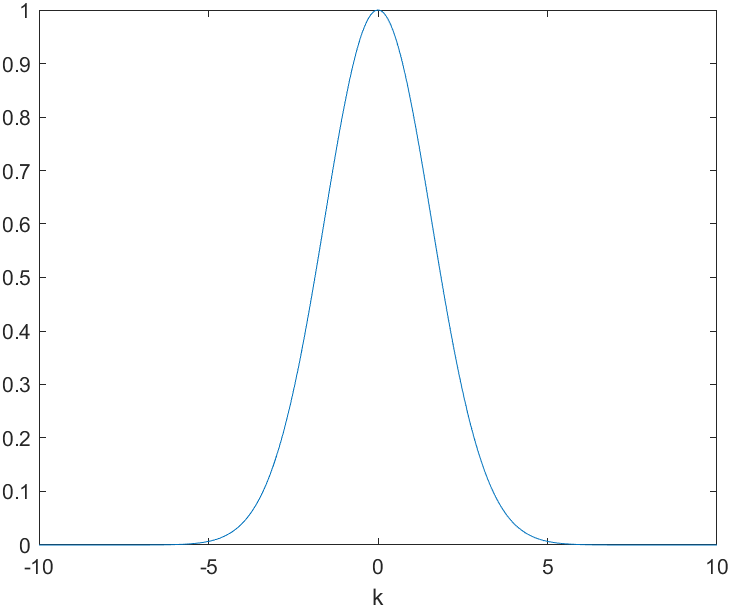
\includegraphics[width=3in]{gauss.png}}
    \caption{Gauss function with $\tau=1$ and $k_0=0$}
\end{figure}
% Algorithm Implementation and Development
\section{Algorithm Implementation and Development}
\subsection{Preparation}
Since we want to vitalize the spectrum in 3-D space by \textbf{isosurface}, we defined some variables and constants for data vitalization, including the space domain, the frequency domain, and Fourier node.

\begin{algorithm}
\begin{algorithmic}
    \STATE{Import data from \texttt{subdata.mat}}
    \STATE{Define the size of spacial domain, $L=10$}
    \STATE{Define the Fourier nodes, $n=64$}
    \STATE{Define the space and frequency domains by \texttt{meshgrid}}
\end{algorithmic}
\caption{Preparation}
\end{algorithm}

\newpage
\subsection{Finding Center Frequencies}
Notice that the data we given is 2-D (262144x49) matrix, therefore, we have to reshape it to 4-D (64x64x64x49) matrix.\\
Next, we transformed acoustic data into frequency domain from space domain. Notice that the spectrum is 3-D, therefore we had to use \texttt{fftn} instead of \texttt{fft} \\
Since we assumed that the noise is white noise, which effect all frequencies by adding a normal distributed random variable with \textbf{zero mean}, therefore we averaged each frequency realizations to eliminate the effect of noise.\\
After denoising the data, we determined the center frequencies by taking the mean of all significant frequencies. \\


\begin{algorithm}
\begin{algorithmic}
    \STATE{Initialize the average matrix}
    \FOR{$j=1:49$}
        \STATE{Reshape the acoustic data at $j^{th}$ time from 1-D to 3-D}
        \STATE{Find the frequency realization at $j^{th}$ time by \texttt{fftn}}
        \STATE{Add the frequency realization to average matrix}
    \ENDFOR
    \STATE{Divides the sum of all frequency realizations by 49}
    \STATE{Find the vertices of averaged frequency realizations by \texttt{isosurface}}
    \STATE{Find the mean of those vertices in each dimensions (x, y, z) coordinates}
\end{algorithmic}
\caption{Finding Center Frequencies}
\end{algorithm}
\begin{figure}[h]
    \centerline{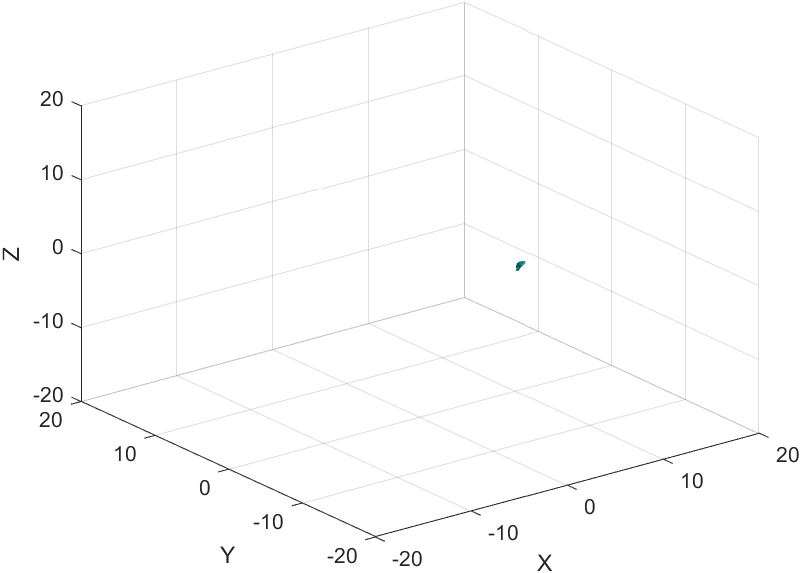
\includegraphics[width=3in]{centf.png}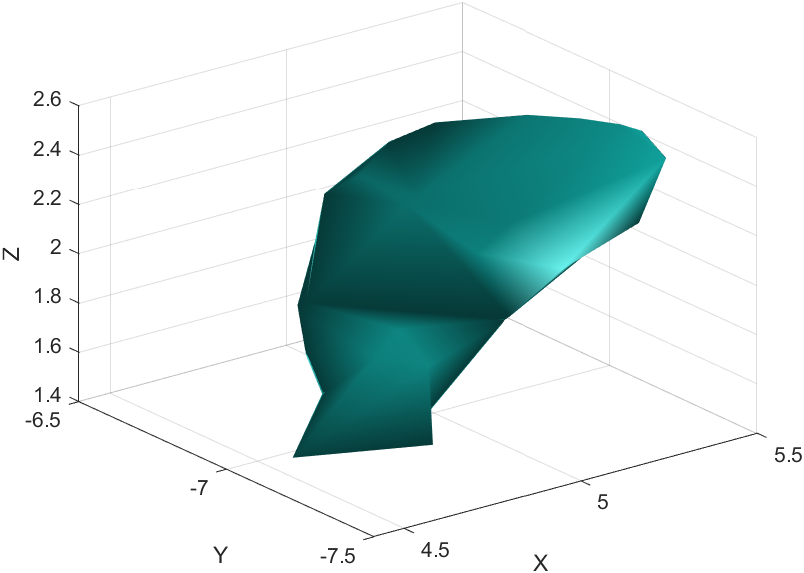
\includegraphics[width=3in]{centf2.png}}
    \caption{Left: The average of all frequency realization \quad Right: Detailed image}
\end{figure}

\newpage
\subsection{Finding the location/path of the submarine}
Since we already knew the center frequencies generated by this new submarine, therefore we could apply filter to focus on the frequencies around the center frequencies. \\
After applying the filter, we transformed the data back to space domain from frequency domain. \\
Since the submarine is a 3-D object, the graph actually gave us a sphere instead of a coordinate. Thus, we used the mean (center) of those vertices again to represent the position of the submarine.

\begin{algorithm}
\begin{algorithmic}
    \STATE{Initialize the Gauss filter matrix for $x,y,z$ coordinates}
    \FOR{$j=1:49$}
        \STATE{Reshape the acoustic data at $j^{th}$ time}
        \STATE{Transform the data into frequency domain by \texttt{fftn}}
        \STATE{Apply the filter on frequency domain}
        \STATE{Transform the data back to space domain by \texttt{ifftn}}
        \STATE{Find the vertices in space domain by \texttt{isosurface}}
        \STATE{Store the mean (center) of those vertices}
    \ENDFOR
    \STATE{Plot the location/path of the submarine}
\end{algorithmic}
\caption{Finding Center Frequencies}
\end{algorithm}
\begin{figure}[h]
    \centerline{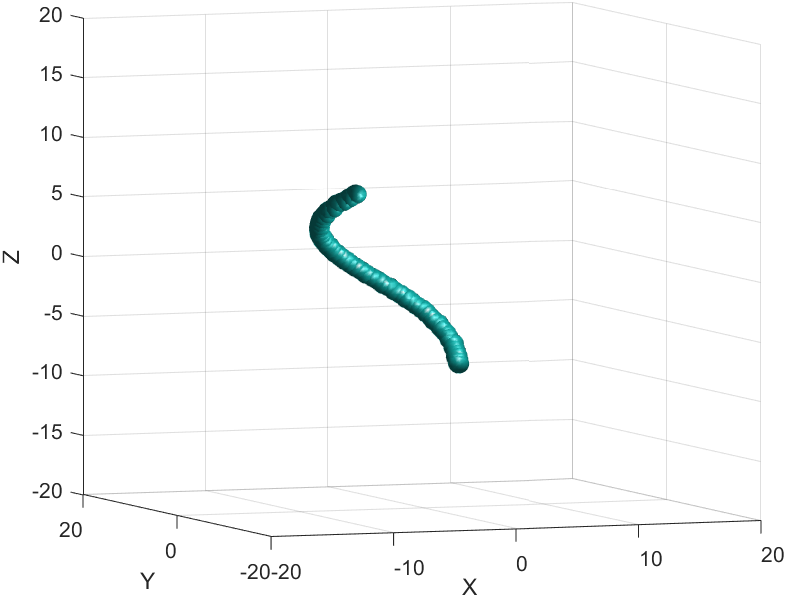
\includegraphics[width=3in]{path1.png}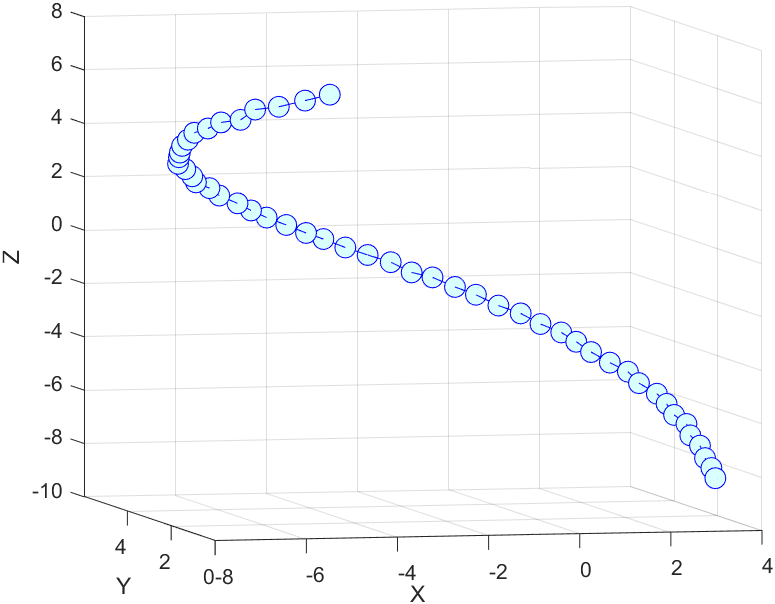
\includegraphics[width=3in]{path2.png}}
    \caption{The spacial realizations at time 1 to 49 (left) \quad The path of submarine (right)}
\end{figure}

\section{Computational Result}
The center frequencies generated by the submarine in $x, y, z$ coordinates are $5.0477, -6.9961, 2.0461$ respectively.
The final location of the submarine is
\begin{center}
    \begin{tabular}{ c c}
        x & y \\
        \hline\hline\\
        -5.0881 & 0.81689   
    \end{tabular}
\end{center}

\section{Summary and Conclusion}
In the study, the first thing we did was eliminating the noise. Notice that the original data is noisy, and we assume that the original data is contaminated by white noise. Thus, we minimized the effect of noise though averaging out at all frequency realization. Figure 2 shows the averaging of spectrum, which seems to have a small cluster centered at $(5, -7, 2)$. By calculating the mean of all vertices, we successfully found the frequency signature generated by this new submarine, which are $5.0477, -6.9961, 2.0461$ in $x,y,z$ coordinates respectively. \\
~\\
Based on the frequency signature, we were able to specify a filter to emphasize on the frequencies around the frequency signature generated by the submarine. Finally, we sent it back to the space domain to determine its location and path, and the Figure 4 below demonstrates the space domain with and without denoising. The last update shows that the $(x,y)$ coordinates of the submarine is $(-5.0881,0.81689)$. 
\begin{figure}[h]
    \centerline{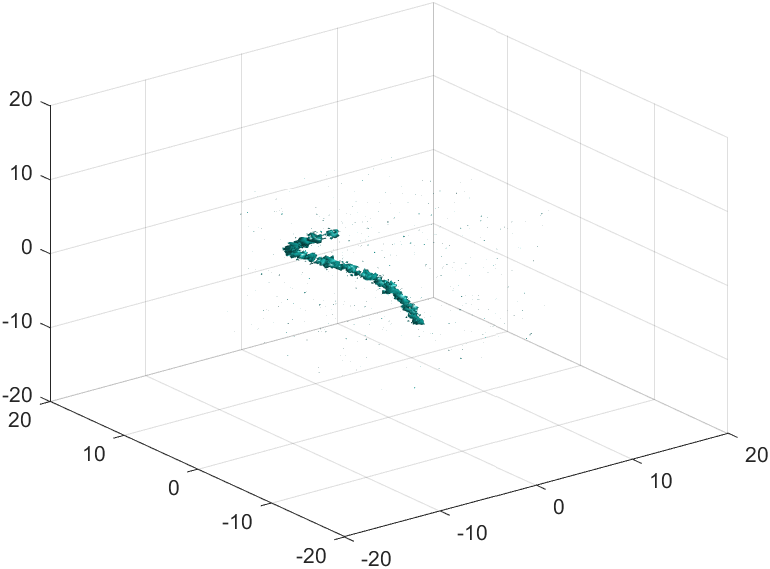
\includegraphics[width=3in]{comp.png}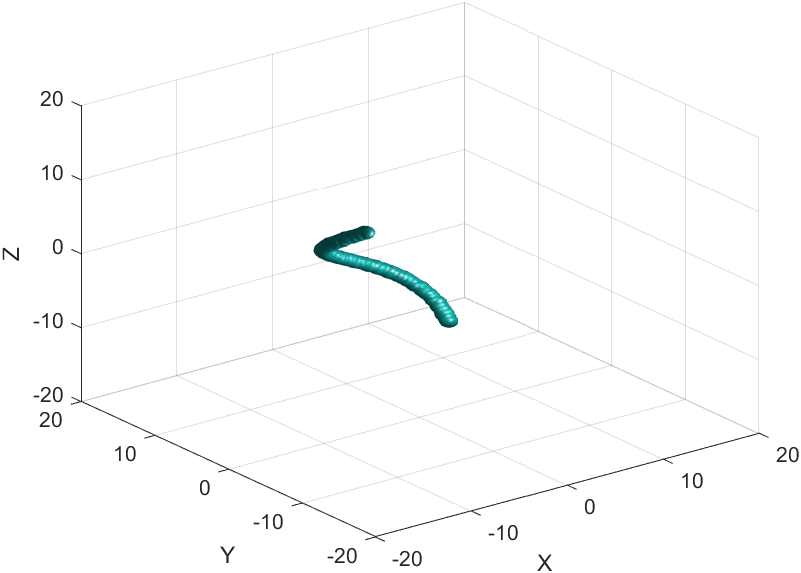
\includegraphics[width=3in]{comp2.png}}
    \caption{Original data(left) \quad Denoised data (right)}
\end{figure}
\newpage
% Appendices
\begin{appendices}

% MATLAB Functions
\section{MATLAB Functions}
Add your important MATLAB functions here with a brief implementation explanation. This is how to make an \textbf{unordered} list:
\begin{itemize}
    \item \texttt{Unt = fftn(Un)} returns the \texttt {multidimensional Fourier transform} of an N-D array using a fast Fourier transform algorithm.
    \item \texttt{Un = ifftn(Unt)} returns the \texttt {multidimensional discrete inverse Fourier transform} of an N-D array using a fast Fourier transform algorithm. 
    \item \texttt{[f,v] = isosurface(...)} returns the faces and vertices in separate arrays.
\end{itemize}

% MATLAB Codes
\newpage
\section{MATLAB Code}

\begin{listing}[H]
  \begin{minted}{matlab} 
%% Clean workspace
clear all; close all; clc

%% setup
load subdata.mat % Imports the data as the 262144x49 (space by time) matrix called subdata

L = 10; % spatial domain
n = 64; % Fourier modes
x2 = linspace(-L,L,n+1); x = x2(1:n); y =x; z = x;
k = (2*pi/(2*L))*[0:(n/2 - 1) -n/2:-1]; ks = fftshift(k);

[X,Y,Z]=meshgrid(x,y,z);
[Kx,Ky,Kz]=meshgrid(ks,ks,ks);

%% problem 1
avg = zeros(64, 64, 64); % Initialize the average matrix
for j=1:49
    Un(:,:,:)=reshape(subdata(:,j),n,n,n); % data at time j
    
    % Plot original data
    % isosurface(X,Y,Z,abs(Un) / M, 0.7);
    % M = max(abs(Un),[],'all');
    % axis([-20 20 -20 20 -20 20]); grid on;
    
    Unt = fftn(Un); % Transforms to frequency domain
    avg = avg + Unt; 
end
% average out at frequency domains
avg = fftshift(abs(avg)) / 49; 
M = max(abs(avg),[],'all');

% Plot the average of the spectrum
% isosurface(Kx,Ky,Kz,abs(avg) / M, 0.7);
% axis([-20 20 -20 20 -20 20]), grid on, drawnow

% calculate the center frequencies of every dimensions.
[f, v] = isosurface(Kx,Ky,Kz,abs(avg) / M, 0.7);
cent_freq = mean(v); 
x_cf = cent_freq(1);
y_cf = cent_freq(2);
z_cf = cent_freq(3);

%% problem 2
% Set up Gauss Filter 
a = 0.2;
x_gauss = exp(-a*(Kx-x_cf).^2); 
y_gauss = exp(-a*(Ky-y_cf).^2); 
z_gauss = exp(-a*(Kz-z_cf).^2); 
gauss_filter = x_gauss .* y_gauss .* z_gauss;


  \end{minted}
\end{listing}
\begin{listing}
  \begin{minted}{matlab}
% Initialize position matrix
positions = zeros(49, 3);
for j=1:49

    Un(:,:,:)=reshape(subdata(:,j),n,n,n); % data at time j
    Unt = gauss_filter .* fftshift(fftn(Un)); % Applies filter on frequency domain
    Un = ifftn(Unt);% Transforms back to spacial domain
    
    % Plot denoised data
    % M = max(abs(Un),[],'all');
    % isosurface(X,Y,Z,abs(Un) / M, 0.7);
    % axis([-20 20 -20 20 -20 20]), grid on, drawnow
    
    % Calculate the center of the submarine at each time.
    [f, v] = isosurface(X,Y,Z,abs(Un) / M, 0.7);
    positions(j,:) = mean(v);
end

% Plot the path of the submarine
% plot3(positions(:,1), positions(:,2), positions(:,3), '-o','Color','b','MarkerSize',10,'MarkerFaceColor','#D9FFFF');

%% problem 3
r = table(positions(49, 1), positions(49, 2))
  \end{minted}
\end{listing}

\end{appendices}

\end{document}
